Recent work has shown that diffusion-based language models (DLLMs) and autoregressive (AR) models can be combined in complementary ways to leverage the strengths of both paradigms. For example, HybridVLA interleaves an AR component for text and image generation with a diffusion component operating on the action space of an embodied agent, allowing a single model to generate rich multimodal descriptions and execute coherent action plans \cite{liu_hybridvla_2025}. In \textbf{Block Diffusion}, fixed-size blocks of tokens are generated by first sampling the initial token autoregressively, then denoising the remainder of the block in parallel via a DLLM, achieving a balance between sequential decoding speed and parallel sampling efficiency \cite{arriola_block_2025}.  

\noindent\textbf{DiffPO} applies a diffusion-style denoising step at inference time to align AR-generated sentences with learned human ``preference'' vectors, reshaping outputs post hoc without retraining the underlying AR model and improving both fluency and alignment metrics \cite{chen_diffpo_2025}. Similarly, Latent Diffusion for Language Generation projects token embeddings into a compact latent space via a compression network and reconstructs tokens through an AR decoder, speeding up sampling while preserving generation quality \cite{lovelace_latent_2023}.  

\noindent In an energy-based approach, \textbf{Energy-Based Diffusion Language Models} train a diffusion process to match a target AR distribution, enabling ``plug and play'' sampling from pretrained AR models via energy gradients and bridging sample efficiency with expressive power \cite{xu_energy-based_2025}. Building on this idea, Speculative Diffusion Decoding uses a fast DLLM as a draft generator to propose multiple continuations in parallel, which are then scored or filtered by an AR model to achieve near AR quality with fewer sequential steps \cite{christopher_speculative_2025}.  

\noindent \textbf{DDPT: Diffusion-Driven Prompt Tuning} uses a DLLM to generate or refine prompts in latent space for a large language model focused on code generation; the prompt is then passed to an AR code generator, and the overall loss computed against ground truth code tunes the prompt space via diffusion \cite{li_ddpt_2025}. On the theoretical side, a \textbf{Unified Hyperschedules Framework} demonstrates that autoregression arises as a special case of diffusion under extreme noise schedules; by modulating noise levels and step counts, one can smoothly interpolate between pure AR and diffusion, or combine them to harness both methods' advantages \cite{fathi_unifying_2025}.  

\noindent \textbf{TEncDM} operates diffusion not on raw tokens but in the continuous encoding space of a frozen LLM encoder–decoder, using cross attention for self-conditioning. This leverages powerful transformer representations while accelerating refinement through parallel diffusion sampling \cite{shabalin_tencdm_2025}.  

\begin{figure}[h!]
    \centering
    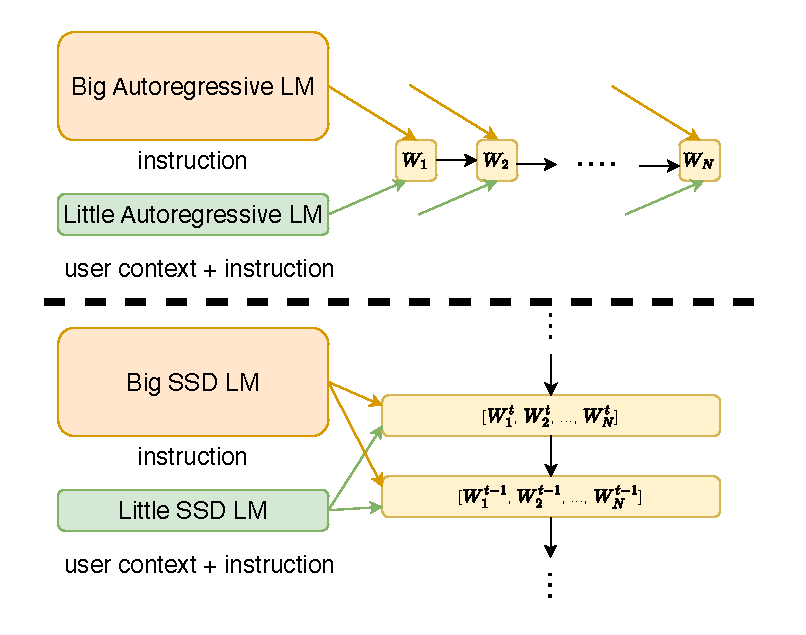
\includegraphics[width=0.5\textwidth]{figs/David_helps_Goliath.pdf}
    \caption[\textit{David helps Goliath} collaboration framework]{%
        \textit{David helps Goliath}~\cite{han_david_2024}: Inference-time collaboration between large and small models. 
        AR models decode token-by-token, while diffusion models refine token blocks iteratively with bidirectional contexts.%
    }
    \label{fig:david_helps_goliath}
\end{figure}

\noindent Finally, \textbf{David helps Goliath} demonstrates DLLM's mutual collaboration advantage over autoregressive counterparts: DLLMs' iterative generation process enables them to reference bidirectional context, therefore, it is easier for different DLLMs to collaborate at the sequence level and yield better quality. Inspired by AR counterparts, the authors incorporate the logits-averaging method to generate a block of tokens at each diffusion step for expert model $\theta_{\mathrm{core}}$ and user model $\theta_{\mathrm{user}}$. Similar to AR counterparts, to increase the pointwise information exchange between the expert generated data and the conditioned generation based on the instruction, a contrastive term $\theta_{\mathrm{user}}$ without input $D_{\text{user}}$ is added.\cite{han_david_2024}

%\begin{equation}
%\label{eq:david_helps_goliath}
%\footnotesize
\small
\begin{align*}
    \boldsymbol{w}_{\text{core-logits}, t}^{c:c+B} &= \operatorname{logits}_{\theta_{\text{core}}}(\boldsymbol{w}^{c:c+B} \mid \boldsymbol{w}_{\text{inst}}, \boldsymbol{w}^{<c}, \Tilde{\boldsymbol{w}}_t^{c:c+B}) \\
    \boldsymbol{w}_{\text{user-logits}, t}^{c:c+B} &= \operatorname{logits}_{\theta_{\text{user}}}(\boldsymbol{w}^{c:c+B} \mid D_{\text{user}}, \boldsymbol{w}_{\text{inst}}, \boldsymbol{w}^{<c}, \Tilde{\boldsymbol{w}}_t^{c:c+B}) \\
    \boldsymbol{w}_{\neg \text{user-logits}, t}^{c:c+B} &= \operatorname{logits}_{\theta_{\text{user}}}(\boldsymbol{w}^{c:c+B} \mid \boldsymbol{w}_{\text{inst}}, \boldsymbol{w}^{<c}, \Tilde{\boldsymbol{w}}_t^{c:c+B}) \\
    \boldsymbol{w}_{\text{logits}, t}^{c:c+B} &= (1-\lambda_{\text{user}}) \boldsymbol{w}_{\text{core-logits}, t}^{c:c+B} \\
    &\quad + \lambda_{\text{user}} (1+\alpha) \boldsymbol{w}_{\text{user-logits}, t}^{c:c+B} - \lambda_{\text{user}} \alpha \boldsymbol{w}_{\neg \text{user-logits}, t}^{c:c+B}
\end{align*}
%\end{equation}


\noindent Together, these approaches illustrate a rich design space for hybrid generation: blockwise and latent space diffusion, post-hoc preference alignment, speculative drafting, prompt tuning, and unified theoretical frameworks. All pointing toward future models that fluidly integrate diffusion and autoregression within a single system.
